\documentclass[DIV=14,titlepage=false]{scrreprt}

%%%%%%%%%%%%%%%%%%%%%%%%%%%%%%%%%%%%%%%%%%%%%%%%%%%%%%%%%%%%%%%%%%%%%%%%%%%%%%%
%                                Basic Packages                               %
%%%%%%%%%%%%%%%%%%%%%%%%%%%%%%%%%%%%%%%%%%%%%%%%%%%%%%%%%%%%%%%%%%%%%%%%%%%%%%%
% Gives us multiple colors.
\usepackage[usenames,dvipsnames,pdftex]{xcolor}
% Lets us style link colors.
\usepackage{hyperref}
% Lets us import images and graphics.
\usepackage{graphicx}
% Lets us use figures in floating environments.
\usepackage{float}
% Lets us create multiple columns.
\usepackage{multicol}
% Gives us better math syntax.
\usepackage{amsmath,amsfonts,mathtools,amsthm,amssymb}
% Lets us strikethrough text.
\usepackage{cancel}
% Lets us edit the caption of a figure.
\usepackage{caption}
% Lets us import pdf directly in our tex code.
\usepackage{pdfpages}
% Lets us do algorithm stuff.
\usepackage[ruled,vlined,linesnumbered]{algorithm2e}
% Gets rid of some errors.
\usepackage{scrhack}
\def\class{article}
\usepackage{geometry}
\geometry{margin=0.9in}
%%%%%%%%%%%%%%%%%%%%%%%%%%%%%%%%%%%%%%%%%%%%%%%%%%%%%%%%%%%%%%%%%%%%%%%%%%%%%%%
%                                Basic Settings                               %
%%%%%%%%%%%%%%%%%%%%%%%%%%%%%%%%%%%%%%%%%%%%%%%%%%%%%%%%%%%%%%%%%%%%%%%%%%%%%%%

%%%%%%%%%%%%%
%  Symbols  %
%%%%%%%%%%%%%

\let\implies\Rightarrow
\let\impliedby\Leftarrow
\let\iff\Leftrightarrow
\let\epsilon\varepsilon

%%%%%%%%%%%%
%  Tables  %
%%%%%%%%%%%%

\setlength{\tabcolsep}{5pt}
\renewcommand\arraystretch{1.5}

%%%%%%%%%%%%%%%%%%%%%%%
%  Center Title Page  %
%%%%%%%%%%%%%%%%%%%%%%%

\usepackage{titling}
\renewcommand\maketitlehooka{\null\mbox{}\vfill}
\renewcommand\maketitlehookd{\vfill\null}

%%%%%%%%%%%%%%%%%%%%%%%%%%%%%%%%%%%%%%%%%%%%%%%%%%%%%%%
%  Create a grey background in the middle of the PDF  %
%%%%%%%%%%%%%%%%%%%%%%%%%%%%%%%%%%%%%%%%%%%%%%%%%%%%%%%

\usepackage{eso-pic}
\newcommand\definegraybackground{
  \definecolor{reallylightgray}{HTML}{FAFAFA}
  \AddToShipoutPicture{
    \ifthenelse{\isodd{\thepage}}{
      \AtPageLowerLeft{
        \put(\LenToUnit{\dimexpr\paperwidth-222pt},0){
          \color{reallylightgray}\rule{222pt}{297mm}
        }
      }
    }
    {
      \AtPageLowerLeft{
        \color{reallylightgray}\rule{222pt}{297mm}
      }
    }
  }
}

%%%%%%%%%%%%%%%%%%%%%%%%
%  Modify Links Color  %
%%%%%%%%%%%%%%%%%%%%%%%%

\hypersetup{
  % Enable highlighting links.
  colorlinks,
  % Change the color of links to blue.
  linkcolor={black},
  % Change the color of citations to black.
  citecolor={black},
  % Change the color of url's to blue with some black.
  urlcolor=blue
}

%%%%%%%%%%%%%%%%%%
% Fix WrapFigure %
%%%%%%%%%%%%%%%%%%

\newcommand{\wrapfill}{\par\ifnum\value{WF@wrappedlines}>0
    \parskip=0pt
    \addtocounter{WF@wrappedlines}{-1}%
    \null\vspace{\arabic{WF@wrappedlines}\baselineskip}%
    \WFclear
\fi}

%%%%%%%%%%%%%%%%%
% Multi Columns %
%%%%%%%%%%%%%%%%%

\let\multicolmulticols\multicols
\let\endmulticolmulticols\endmulticols

\RenewDocumentEnvironment{multicols}{mO{}}
{%
  \ifnum#1=1
    #2%
  \else % More than 1 column
    \multicolmulticols{#1}[#2]
  \fi
}
{%
  \ifnum#1=1
\else % More than 1 column
  \endmulticolmulticols
\fi
}

\newlength{\thickarrayrulewidth}
\setlength{\thickarrayrulewidth}{5\arrayrulewidth}

%%%%%%%%%%%%%%%%%%%%
%  Import Figures  %
%%%%%%%%%%%%%%%%%%%%

\usepackage{import}
\pdfminorversion=7

% EXAMPLE:
% 1. \incfig{limit-graph}
% 2. \incfig[0.4]{limit-graph}
% Parameters:
% 1. The figure name. It should be located in figures/NAME.tex_pdf.
% 2. (Optional) The width of the figure. Example: 0.5, 0.35.
\newcommand\incfig[2][1]{%
  \def\svgwidth{#1\columnwidth}
  \import{./figures/}{#2.pdf_tex}
}

\begingroup\expandafter\expandafter\expandafter\endgroup
\expandafter\ifx\csname pdfsuppresswarningpagegroup\endcsname\relax
\else
  \pdfsuppresswarningpagegroup=1\relax
\fi

%%%%%%%%%%%%%
%  Correct  %
%%%%%%%%%%%%%

% EXAMPLE:
% 1. \correct{INCORRECT}{CORRECT}
% Parameters:
% 1. The incorrect statement.
% 2. The correct statement.
\definecolor{correct}{HTML}{009900}
\newcommand\correct[2]{{\color{red}{#1 }}\ensuremath{\to}{\color{correct}{ #2}}}



\newcommand{\R}{\mathbb{R}}
\newcommand{\Z}{\mathbb{Z}}
\newcommand{\E}{\mathbb{E}}
\newcommand{\B}{\ensuremath{\mathcal{B}}}
\newcommand{\X}{\ensuremath{\mathcal{X}}}
\newcommand{\Y}{\ensuremath{\mathcal{Y}}}
\newcommand{\mA}{\ensuremath{\mathbf{A}}}
\newcommand{\mB}{\ensuremath{\mathbf{B}}}
\newcommand{\mC}{\ensuremath{\mathbf{C}}}
\newcommand{\mD}{\ensuremath{\mathbf{D}}}
\newcommand{\mX}{\ensuremath{\mathbf{X}}}
\newcommand{\mY}{\ensuremath{\mathbf{Y}}}
\newcommand{\mx}{\ensuremath{\mathbf{x}}}
\newcommand{\my}{\ensuremath{\mathbf{y}}}
\newcommand{\mI}{\ensuremath{\mathbf{I}}}
\newcommand{\mi}{\ensuremath{\mathbf{\iota}}}
\newcommand{\mmu}{\ensuremath{\mathbf{\mu}}}
\newcommand{\mc}{\ensuremath{\mathbf{c}}}
\newcommand{\mSigma}{\ensuremath{\mathbf{\Sigma}}}
\newcommand{\mzero}{\ensuremath{\mathbf{0}}}
\newcommand{\independent}{\perp\!\!\!\!\perp} 
\setlength{\parindent}{0pt}
%%%%%%%%%%%%%%%%%%%%%%%%%%%%%%%%%%%%%%%%%%%%%%%%%%%%%%%%%%%%%%%%%%%%%%%%%%%%%%%
%                                 Environments                                %
%%%%%%%%%%%%%%%%%%%%%%%%%%%%%%%%%%%%%%%%%%%%%%%%%%%%%%%%%%%%%%%%%%%%%%%%%%%%%%%

\usepackage{varwidth}
\usepackage{thmtools}
\usepackage[most,many,breakable]{tcolorbox}

\tcbuselibrary{theorems,skins,hooks}
\usetikzlibrary{arrows,calc,shadows.blur}

%%%%%%%%%%%%%%%%%%%
%  Define Colors  %
%%%%%%%%%%%%%%%%%%%

\definecolor{myblue}{RGB}{45, 111, 177}
\definecolor{mygreen}{RGB}{56, 140, 70}
\definecolor{myred}{RGB}{199, 68, 64}
\definecolor{mypurple}{RGB}{197, 92, 212}

\definecolor{definition}{HTML}{228b22}
\definecolor{theorem}{HTML}{00007B}
\definecolor{example}{HTML}{2A7F7F}
\definecolor{definition}{HTML}{228b22}
\definecolor{prop}{HTML}{191971}
\definecolor{lemma}{HTML}{983b0f}
\definecolor{exercise}{HTML}{88D6D1}

\colorlet{definition}{mygreen!85!black}
\colorlet{claim}{mygreen!85!black}
\colorlet{corollary}{mypurple!85!black}
\colorlet{proof}{theorem}

%%%%%%%%%%%%%%%%%%%%%%
%  Helpful Commands  %
%%%%%%%%%%%%%%%%%%%%%%

% EXAMPLE:
% 1. \createnewtheoremstyle{thmdefinitionbox}{}{}
% 2. \createnewtheoremstyle{thmtheorembox}{}{}
% 3. \createnewtheoremstyle{thmproofbox}{qed=\qedsymbol}{
%       rightline=false, topline=false, bottomline=false
%    }
% Parameters:
% 1. Theorem name.
% 2. Any extra parameters to pass directly to declaretheoremstyle.
% 3. Any extra parameters to pass directly to mdframed.
\newcommand\createnewtheoremstyle[3]{
  \declaretheoremstyle[
  headfont=\bfseries\sffamily, bodyfont=\normalfont, #2,
  mdframed={
    #3,
  },
  ]{#1}
}

% EXAMPLE:
% 1. \createnewcoloredtheoremstyle{thmdefinitionbox}{definition}{}{}
% 2. \createnewcoloredtheoremstyle{thmexamplebox}{example}{}{
%       rightline=true, leftline=true, topline=true, bottomline=true
%     }
% 3. \createnewcoloredtheoremstyle{thmproofbox}{proof}{qed=\qedsymbol}{backgroundcolor=white}
% Parameters:
% 1. Theorem name.
% 2. Color of theorem.
% 3. Any extra parameters to pass directly to declaretheoremstyle.
% 4. Any extra parameters to pass directly to mdframed.
\newcommand\createnewcoloredtheoremstyle[4]{
  \declaretheoremstyle[
  headfont=\bfseries\sffamily\color{#2}, bodyfont=\normalfont, #3,
  mdframed={
    linewidth=2pt,
    rightline=false, leftline=true, topline=false, bottomline=false,
    linecolor=#2, backgroundcolor=#2!5, #4,
  },
  ]{#1}
}

%%%%%%%%%%%%%%%%%%%%%%%%%%%%%%%%%%%
%  Create the Environment Styles  %
%%%%%%%%%%%%%%%%%%%%%%%%%%%%%%%%%%%

\makeatletter
\@ifclasswith\class{nocolor}{
  % Environments without color.

  \createnewtheoremstyle{thmdefinitionbox}{}{}
  \createnewtheoremstyle{thmtheorembox}{}{}
  \createnewtheoremstyle{thmexamplebox}{}{}
  \createnewtheoremstyle{thmclaimbox}{}{}
  \createnewtheoremstyle{thmcorollarybox}{}{}
  \createnewtheoremstyle{thmpropbox}{}{}
  \createnewtheoremstyle{thmlemmabox}{}{}
  \createnewtheoremstyle{thmexercisebox}{}{}
  \createnewtheoremstyle{thmdefinitionbox}{}{}
  \createnewtheoremstyle{thmquestionbox}{}{}
  \createnewtheoremstyle{thmsolutionbox}{}{}

  \createnewtheoremstyle{thmproofbox}{qed=\qedsymbol}{}
  \createnewtheoremstyle{thmexplanationbox}{}{}
}{
  % Environments with color.

  \createnewcoloredtheoremstyle{thmdefinitionbox}{definition}{}{}
  \createnewcoloredtheoremstyle{thmtheorembox}{theorem}{}{}
  \createnewcoloredtheoremstyle{thmexamplebox}{example}{}{
    rightline=true, leftline=true, topline=true, bottomline=true
  }
  \createnewcoloredtheoremstyle{thmclaimbox}{claim}{}{}
  \createnewcoloredtheoremstyle{thmcorollarybox}{corollary}{}{}
  \createnewcoloredtheoremstyle{thmpropbox}{prop}{}{}
  \createnewcoloredtheoremstyle{thmlemmabox}{lemma}{}{}
  \createnewcoloredtheoremstyle{thmexercisebox}{exercise}{}{}

  \createnewcoloredtheoremstyle{thmproofbox}{proof}{qed=\qedsymbol}{backgroundcolor=white}
  \createnewcoloredtheoremstyle{thmexplanationbox}{example}{qed=\qedsymbol}{backgroundcolor=white}
}
\makeatother

%%%%%%%%%%%%%%%%%%%%%%%%%%%%%
%  Create the Environments  %
%%%%%%%%%%%%%%%%%%%%%%%%%%%%%

\declaretheorem[numberwithin=section, style=thmtheorembox,     name=Theorem]{theorem}
\declaretheorem[numbered=no,          style=thmexamplebox,     name=Example]{example}
\declaretheorem[numberwithin=section, style=thmclaimbox,       name=Claim]{claim}
\declaretheorem[numberwithin=section, style=thmcorollarybox,   name=Corollary]{corollary}
\declaretheorem[numberwithin=section, style=thmpropbox,        name=Proposition]{prop}
\declaretheorem[numberwithin=section, style=thmlemmabox,       name=Lemma]{lemma}
\declaretheorem[numberwithin=section, style=thmexercisebox,    name=Exercise]{exercise}
\declaretheorem[numbered=no,          style=thmproofbox,       name=Proof]{replacementproof}
\declaretheorem[numbered=no,          style=thmexplanationbox, name=Proof]{expl}

\makeatletter
\@ifclasswith\class{nocolor}{
  % Environments without color.

  \newtheorem*{note}{Note}

  \declaretheorem[numberwithin=section, style=thmdefinitionbox, name=Definition]{definition}
  \declaretheorem[numberwithin=section, style=thmquestionbox,   name=Question]{question}
  \declaretheorem[numberwithin=section, style=thmsolutionbox,   name=Solution]{solution}
}{
  % Environments with color.

  \newtcbtheorem[number within=section]{Definition}{Definition}{
    enhanced,
    before skip=2mm,
    after skip=2mm,
    colback=red!5,
    colframe=red!80!black,
    colbacktitle=red!75!black,
    boxrule=0.5mm,
    attach boxed title to top left={
      xshift=1cm,
      yshift*=1mm-\tcboxedtitleheight
    },
    varwidth boxed title*=-3cm,
    boxed title style={
      interior engine=empty,
      frame code={
        \path[fill=tcbcolback]
        ([yshift=-1mm,xshift=-1mm]frame.north west)
        arc[start angle=0,end angle=180,radius=1mm]
        ([yshift=-1mm,xshift=1mm]frame.north east)
        arc[start angle=180,end angle=0,radius=1mm];
        \path[left color=tcbcolback!60!black,right color=tcbcolback!60!black,
        middle color=tcbcolback!80!black]
        ([xshift=-2mm]frame.north west) -- ([xshift=2mm]frame.north east)
        [rounded corners=1mm]-- ([xshift=1mm,yshift=-1mm]frame.north east)
        -- (frame.south east) -- (frame.south west)
        -- ([xshift=-1mm,yshift=-1mm]frame.north west)
        [sharp corners]-- cycle;
      },
    },
    fonttitle=\bfseries,
    title={#2},
    #1
  }{def}

  \NewDocumentEnvironment{definition}{O{}O{}}
    {\begin{Definition}{#1}{#2}}{\end{Definition}}

  \newtcolorbox{note}[1][]{%
    enhanced jigsaw,
    colback=gray!20!white,%
    colframe=gray!80!black,
    size=small,
    boxrule=1pt,
    title=\textbf{Note:-},
    halign title=flush center,
    coltitle=black,
    breakable,
    drop shadow=black!50!white,
    attach boxed title to top left={xshift=1cm,yshift=-\tcboxedtitleheight/2,yshifttext=-\tcboxedtitleheight/2},
    minipage boxed title=1.5cm,
    boxed title style={%
      colback=white,
      size=fbox,
      boxrule=1pt,
      boxsep=2pt,
      underlay={%
        \coordinate (dotA) at ($(interior.west) + (-0.5pt,0)$);
        \coordinate (dotB) at ($(interior.east) + (0.5pt,0)$);
        \begin{scope}
          \clip (interior.north west) rectangle ([xshift=3ex]interior.east);
          \filldraw [white, blur shadow={shadow opacity=60, shadow yshift=-.75ex}, rounded corners=2pt] (interior.north west) rectangle (interior.south east);
        \end{scope}
        \begin{scope}[gray!80!black]
          \fill (dotA) circle (2pt);
          \fill (dotB) circle (2pt);
        \end{scope}
      },
    },
    #1,
  }

  \newtcbtheorem{Question}{Question}{enhanced,
    breakable,
    colback=white,
    colframe=myblue!80!black,
    attach boxed title to top left={yshift*=-\tcboxedtitleheight},
    fonttitle=\bfseries,
    title=\textbf{Question:-},
    boxed title size=title,
    boxed title style={%
      sharp corners,
      rounded corners=northwest,
      colback=tcbcolframe,
      boxrule=0pt,
    },
    underlay boxed title={%
      \path[fill=tcbcolframe] (title.south west)--(title.south east)
      to[out=0, in=180] ([xshift=5mm]title.east)--
      (title.center-|frame.east)
      [rounded corners=\kvtcb@arc] |-
      (frame.north) -| cycle;
    },
    #1
  }{def}

  \NewDocumentEnvironment{question}{O{}O{}}
  {\begin{Question}{#1}{#2}}{\end{Question}}

  \newtcolorbox{Solution}{enhanced,
    breakable,
    colback=white,
    colframe=mygreen!80!black,
    attach boxed title to top left={yshift*=-\tcboxedtitleheight},
    title=\textbf{Solution:-},
    boxed title size=title,
    boxed title style={%
      sharp corners,
      rounded corners=northwest,
      colback=tcbcolframe,
      boxrule=0pt,
    },
    underlay boxed title={%
      \path[fill=tcbcolframe] (title.south west)--(title.south east)
      to[out=0, in=180] ([xshift=5mm]title.east)--
      (title.center-|frame.east)
      [rounded corners=\kvtcb@arc] |-
      (frame.north) -| cycle;
    },
  }

  \NewDocumentEnvironment{solution}{O{}O{}}
  {\vspace{-10pt}\begin{Solution}{#1}{#2}}{\end{Solution}}
}
\makeatother

%%%%%%%%%%%%%%%%%%%%%%%%%%%%
%  Edit Proof Environment  %
%%%%%%%%%%%%%%%%%%%%%%%%%%%%

\renewenvironment{proof}[1][\proofname]{\vspace{-10pt}\begin{replacementproof}}{\end{replacementproof}}
\newenvironment{explanation}[1][\proofname]{\vspace{-10pt}\begin{expl}}{\end{expl}}

\theoremstyle{definition}

\newtheorem*{notation}{Notation}
\newtheorem*{previouslyseen}{As previously seen}
\newtheorem*{problem}{Problem}
\newtheorem*{observe}{Observe}
\newtheorem*{property}{Property}
\newtheorem*{intuition}{Intuition}

\setuptoc{toc}{leveldown}

\begin{document}
\vspace{-10pt}
\chapter{Basic Probability. Conditional expectation function.}
\section{Random Variables}

\begin{definition}[Cumulative distribution function]
  The cumulative distribution function of X is  defined as $ F_X(x) \equiv P(X \leq x) $. 
  A function $ F $ is a cdf iff:
  \begin{enumerate}
  \item $ \lim_{x \to -\infty} F(x) = 0 $ and $ \lim_{x \to \infty} F(x) = 1 $;
  \item $ F (\cdot) $ nondecreasing;
  \item $ F (\cdot) $ right-continuous; i.e., $ \forall x_0 $, $ \lim_{x \downarrow x_0} F(x) = F(x_0) $.
  \end{enumerate}
\end{definition}
\vspace{5pt}
\begin{definition}[Probability density function]
  For a continuous r.v., $ f_X (x) $ defined as the function which satisfies $ F_X(x) = \int_{-\infty}^{x} f_X(t) \, dt $ for all $ x $. A function $ f_X $ is a pdf iff:
  \begin{enumerate}
  \item $ \forall x $, $ f_X(x) \geq 0 $;
  \item $ \int_\R f_X(x) \, dx = 1 $.
  \end{enumerate}
\end{definition}
\vspace{5pt}
$ f_X $ gives the probability of any event: $ P (X \in B) = \int_\R 1_{(x \in B)} f_X(x) \, dx $.

A continuous (in all dimensions) random vector $ X $ has joint pdf\index{Joint pdf} $ f_X(x_1, \dotsc, x_n) $ iff $ \forall A \subseteq \R^n, $ $ P(X \in A) = \idotsint_A f_X(x_1, \dotsc, x_n) \, dx_1 \dotsm dx_n $.
\vspace{5pt}
\begin{exercise}
  Show that the standard normal density integrates to unity by showing (when \( u > 0 \)):
  \[
\frac{1}{\sqrt{2\pi}} \int_{-\infty}^{\infty} e^{-\frac{1}{2}u y^2} dy = \frac{1}{\sqrt{u}}.
\]
\end{exercise}
\begin{solution}
\[\left[
\int_{-\infty}^{\infty} \frac{1}{\sqrt{2\pi}} e^{-\frac{1}{2}y^2} dy
\right]
\left[
\int_{-\infty}^{\infty} \frac{1}{\sqrt{2\pi}} e^{-\frac{1}{2}x^2} dx
\right] 
= \frac{1}{2\pi} \int_{-\infty}^{\infty} \int_{-\infty}^{\infty} e^{-\frac{1}{2}(x^2+y^2)} dxdy.
\]
By changing to polar coordinates, $x^2+y^2=r^2$ and $dxdy=rdrd\theta$. Thus, the desired integral becomes:
\[ \frac{1}{2\pi} \int_{0}^{2\pi} \int_{0}^{\infty} e^{-\frac{1}{2}ur^2} rdrd\theta = \frac{1}{u}\]
Setting $u=1$ yields the desired result.
\end{solution}
\begin{definition}[$\tau$-th quantile]
  Let \( X \) be a random variable with distribution function \( F_X \). The \(\tau\)-th quantile of \( X \) is defined as the value \( x_\tau \) such that
\[ F_X^{-1}(\tau) = \inf\{ x : F_X(x) \geq \tau \} \]
where \( 0 \leq \tau \leq 1 \).
\end{definition}
\vspace{5pt}
\textbf{Why inf and not min?}\\
Because $F$ is right-continuous and nondecreasing, the superlevel sets of F are of the form $[a,\infty]$ where $a>-\infty$ or else the entire real line. When the superlevel set is the whole line, there is no min (among the reals), while the inf is -$ \infty$. For a = +$ \infty$ the superlevel set is empty and so the inf = +$\infty$. These cases can potentially arise when $\tau=0$ or $\tau = 1$ respectively.
\textit{If $\tau \in (0,1)$ then we can replace inf with min.}\\
If $X$ is discrete, then using minimum and infimum are equivalent, since the support is finite and attains a minimum at some point. However, a contimuous $X$ with infinite support will not achieve a minimum, hence the infimum is needed.

\begin{example}
The CDF of an Exponential distribution with parameter \(\lambda\) is given by
  \[
  F(x; \lambda) = 
  \begin{cases} 
  1 - e^{-\lambda x} & x \geq 0, \\
  0 & x < 0.
  \end{cases}
  \]
  The quantile function for Exponential(\(\lambda\)) is derived by finding the value of \(Q\) for which \(1 - e^{-\lambda Q} = p\):
  \[
  Q(p; \lambda) = \frac{-\ln(1 - p)}{\lambda},
  \]
  for \(0 \leq p < 1\). The quartiles are therefore:
  
  \begin{itemize}
    \item First quartile (\(p = 1/4\)): \( -\ln(3/4) / \lambda \)
    \item Median (\(p = 1/2\)): \( -\ln(1/2) / \lambda \)
    \item Third quartile (\(p = 3/4\)): \( -\ln(1/4) / \lambda \).
  \end{itemize}

\end{example}
\vspace{5pt}
\begin{definition}[Expectation]
  For a function \( g \), the expectation of \( g(X) \) is defined as \( \mathbb{E}g(X) = \int_{-\infty}^{\infty} g(x)f(x) \, dx \).
\end{definition}
\vspace{5pt}

\begin{exercise}
  Suppose that Y is a continuous random variable with density $f(y$) that is positive only if $y \geq 0$. If $F(y)$ is the distribution function, show that \[ \E(Y)= \int_{0}^{\infty} [1 - F(y)]dy \]
\end{exercise}
\begin{solution}
  \[E(Y) = \int_{0}^{\infty} yf(y)dy = \int_{0}^{\infty} \left( \int_{0}^{y} dt \right) f(y)dy = \int_{0}^{\infty} \left( \int_{t}^{\infty} f(y)dy \right) dt \] \[ = \int_{0}^{\infty} P(Y > y)dy = \int_{0}^{\infty} [1 - F(y)]dy\]

\end{solution}
\begin{definition}[Moment]
   For $ n \in \Z $, the $ n $th moment of $ X $ is $ \mu_{n}' \equiv \E X^n $. Also denote $ \mu_{1}' = \E X $ as $ \mu $. The $ n $th central moment is $ \mu_n \equiv \E(X - \mu)^n $.
\end{definition}

Two different distributions \textit{can} have all the same moments, but only if the variables have unbounded support sets. Note that $\E X^n$ may not exist (the integral might be infinite), then we say the $n$th moment does not exist.

\textbf{Notable moments and properties:}
\begin{itemize}
  \item The first raw moment is the mean, $\mu = \E [X]$
  \begin{itemize}
    \item $ \E [a g_1(X) + b g_2(X) + c] = a \E(g_1(X)) + b \E(g_2(X)) + c $ (i.e., expectation is a linear operator)
    \item The mean is the MSE minimizing predictor for $ X $; i.e., $ \min_b \E (X - b)^2 = \E (X - \E X)^2 $
    \item If $ X_1, \dotsc , X_n $ mutually independent, then $ \E [ g_1(X_1) \cdot \dotsb \cdot g_n(X_n) ] = \E [ g_1(X_1)] \cdot \dotsb \cdot \E [g_n(X_n) ] $.
  \end{itemize}
  \item The second central moment is the variance, $\E [(x-\mu)^2]$
  \begin{itemize}
    \item $Var(aX + bY) = a^2 VarX + b^2 VarY + 2ab Cov(X,Y) $
    \item $\text{Var}(Y) = \E [\text{Var}(Y|X)] + \text{Var}(\E [Y|X])$ (i.e.: residual variance + regression variance)
    \item $ Var \mX \equiv \E [ \mX \mX' ] - \E [ \mX ] \E [ \mX ]' $
    \item $ Var ( \mX + \mY ) = Var ( \mX ) + Cov ( \mX , \mY ) + Cov ( \mX , \mY )' + Var ( \mY ) $;
    \item $ Var (\mA \mX) = \mA Var ( \mX ) \mA' $.
    \item $ Cov (\mA \mX, \mB \mY) = \mA Cov (\mX, \mY) \mB' $;
    \item $ Cov (\mX, \mY) = Cov ( \mY , \mX )' $.
  
  \end{itemize}
  \item The third central moment is the measure of lopsideness of the distribution. When standardised by the standard deviation it is known as the skewness. Any symmetric distribution will have skewness of 0.
  \item The fourth central moment is a measure of the heaviness of the tail. When standardised by the standard deviation, it is known as the kurtosis:
  \[
  \text{Kurt}[X] = \E\left[ \left( \frac{X - \mu}{\sigma} \right)^4 \right]= \frac{\mu_4}{\mu^2_2}.
  \]
\end{itemize}

\begin{example}
  Find \( \mu_n' \) for the uniform random variable with \( \theta_1 = 0 \) and \( \theta_2 = \theta \).
\\
  By definition,
  \[
  \mu_n' = E(Y^n) = \int_{-\infty}^{\infty} y^n f(y) \, dy = \int_{0}^{\theta} y^n \left( \frac{1}{\theta} \right) dy = \frac{y^{n+1}}{\theta(n + 1)} \Bigg|_0^{\theta} = \frac{\theta^n}{n + 1}.
  \]

  Thus,
  \[
  \mu_1' = \mu = \frac{\theta}{2}, \quad \mu_2' = \frac{\theta^2}{3}, \quad \mu_3' = \frac{\theta^3}{4},
  \]
  and so on.
\end{example}
\section{Common Distributions}

\subsection*{Normal (Gaussian)}
PDF: \[ \displaystyle f(x|\mu,\sigma^2) = \frac{1}{\sqrt{2\pi\sigma^2}} e^{-\frac{(x-\mu)^2}{2\sigma^2}} \]
\vspace{10pt}

\begin{minipage}[c]{0.5\textwidth}
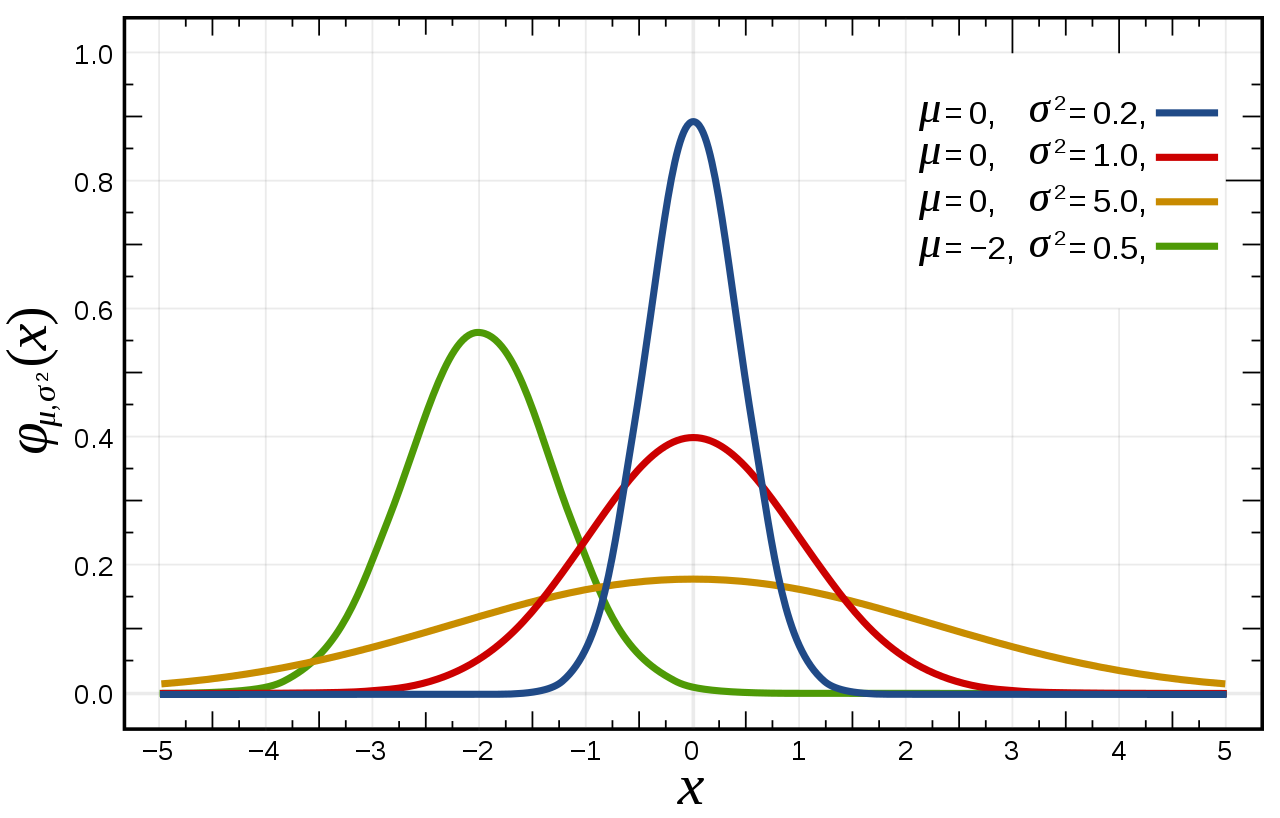
\includegraphics[width=\textwidth]{./Images/univariateNormal.png}
\end{minipage}
\hfill
\begin{minipage}[c]{0.45\textwidth}
  \begin{itemize}
    \item $ \mathbb{E}[X] = \mu $ \\
    $ \mathbb{E}[(X - \mu)] = 0 $
    \item $ \mathbb{E}[X^2] = \mu^2 + \sigma^2 $ \\
    $ \mathbb{E}[(X - \mu)^2] = \sigma^2 $
    \item $ \mathbb{E}[X^3] = \mu^3 + 3\mu\sigma^2 $ \\
    $ \mathbb{E}[(X - \mu)^3] = 0 $
    \item $ \mathbb{E}[X^4] = \mu^4 + 6\mu^2\sigma^2 + 3\sigma^4 $ \\
    $ \mathbb{E}[(X - \mu)^4] = 3\sigma^4 $
  \end{itemize}
  
\end{minipage}
\textbf{Properties}
\begin{itemize}
  \item The distribution is entirely characterised by the first two moments
  \item Square of standard normal is $ \chi^2_1 $.
  \item If $ X \sim N (\mu, \sigma^2) $, $ Y \sim N (\gamma, \tau^2) $, and $ X \independent Y $, then $ X + Y \sim N (\mu + \gamma, \sigma^2 + \tau^2) $ (i.e., independent normals are additive in mean and variance).
  \item For a standard normal: $ \E [Z^k] = 0 $ if $ k $ odd, $ \E [Z^k] = 1 \cdot 3 \cdot 5 \dotsm (n-1) $ if $ k $ even.
  \item Ratio of independent standard normals is Cauchy ($ \sigma = 1 $, $ \theta = 0 $)
\end{itemize}

\begin{lemma}[Stein's Lemma]
  If $ g(\cdot) $ is differentiable with $ \E | g'(X)| < \infty $, then $ \E [g(X)(X - \mu)] = \sigma^2 \E g'(X) $.
\end{lemma}

\begin{proof}[Standard Normal]
  We shall prove in the case of a standard normal: $\phi(x) = \frac{1}{\sqrt{2\pi}} e^{-x^2/2}$
\\
  Since $\int x \exp(-x^2/2) \, dx = - \exp(-x^2/2)$ we get from integration by parts:
  
  $E[g(X)X] = \frac{1}{\sqrt{2\pi}} \int g(x) x \exp(-x^2/2) \, dx = \frac{1}{\sqrt{2\pi}} \int g'(x) \exp(-x^2/2) \, dx = E[g'(X)].$
\end{proof}

\subsection*{Multivariate Normal}
PDF: \[ \displaystyle \frac{1}{\sqrt{(2\pi)^k|\boldsymbol{\Sigma}|}} e^{-\frac{1}{2}(\mathbf{x}-\boldsymbol{\mu})^\top\boldsymbol{\Sigma}^{-1}(\mathbf{x}-\boldsymbol{\mu})} \]
where $ \mathbf{\mu} = \E [\mX] $ and $ \mathbf{\Sigma}_{ij} = Cov (X_i, X_j) $
\vspace{10pt}

\begin{minipage}[c]{0.5\textwidth}
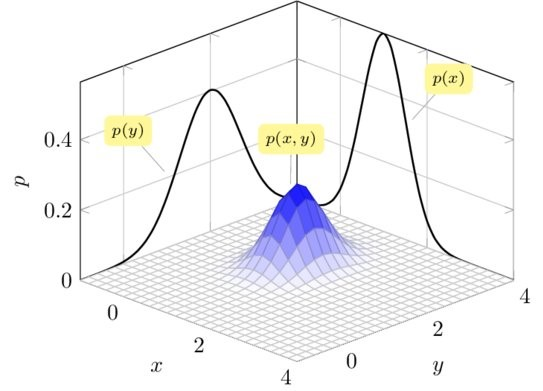
\includegraphics[width=\textwidth]{./Images/bivariateNormal.jpeg}
\end{minipage}
\hfill
\begin{minipage}[c]{0.45\textwidth}
  \textbf{Bivariate Case}
  \begin{itemize}
    \item $\boldsymbol{\mu} = \begin{pmatrix} \mu_X \\ \mu_Y \end{pmatrix}$
    \item $\boldsymbol{\Sigma} = \begin{pmatrix} \sigma_X^2 & \rho\sigma_X\sigma_Y \\ \rho\sigma_X\sigma_Y & \sigma_Y^2 \end{pmatrix}$
  \end{itemize}
  
\end{minipage}\\\\

\textbf{Properties}
\begin{itemize}
  \item A linear transformation of a normal is normal: if $ \mX \sim N_p (\mmu, \mSigma) $, then for any $ \mA \in \R^{q \times p} $ with full row rank ($\implies q \leq p $), and any $ \mathbf{b} \in \R^q $, we have $ \mA \mX + \mathbf{b} \sim N_q (\mA \mmu + \mathbf{b} , \mA \mSigma \mA' ) $. In particular, $ \mSigma^{-1/2} (\mX - \mmu) \sim N (\mzero, \mI)$.
  \item The following transformations of $ \mX \sim N_p (\mmu, \mSigma) $ are independent iff $ \mA \mSigma \mB' = Cov (\mA \mX , \mB \mX) = \mzero $:
  \begin{itemize}
  \item $ \mA \mX \sim N (\mA \mmu , \mA \mSigma \mA') $ and $ \mB \mX \sim N (\mB \mmu , \mB \mSigma \mB') $,
  \item $ \mA \mX \sim N (\mA \mmu , \mA \mSigma \mA') $ and $ \mX' \mB \mX \sim \chi^2_{rk (\mB \Sigma)} $ (where $ \mB \mSigma $ is an idempotent matrix),
  \item $ \mX' \mA \mX \sim \chi^2_{rk (\mA \Sigma)} $ and $ \mX' \mB \mX \sim \chi^2_{rk (\mB \Sigma)} $ (where $ \mA \mSigma $ and $ \mB \mSigma $ are idempotent matrices).
  \end{itemize}
  \item If $X$ and $Y$ are both normal and independent, this implies they are jointly normally distributed (i.e. $(X,Y)$ is multivariate normal). However, a pair of jointly normal distributed variables need not be independent (would only be of if uncorrelated, $\rho=0$).
  \item Independence and zero-covariance are equivalent for linear functions of normally distributed r.v.s.
\end{itemize}

\begin{example}[Individual normality $\not\implies$ joint normality] Consider $X \sim N(0,1)$, and: \[
  Y= 
\begin{cases}
  X,& \text{if } |X| \leq c\\
  -X,& \text{if } |X| > c
\end{cases}
\hspace{10pt}
\text{where $c>0$}
\]
When \( c \) is very small, \( \text{corr}(X, Y) \approx -1\) and when \( c \) is very large, \( \text{corr}(X, Y) \approx 1 \). If the correlation is a continuous function of \( c \), then there exists some \( c \) such that the correlation is \( 0 \). $X$ and $Y$ are uncorrelated, but clearly not independent since $X$ completely determines $Y$. To show $Y$ is normal:

\[
\begin{aligned}
P(Y \leq x) &= P(|X| < c \text{ and } X \leq x) + P(|X| > c \text{ and } -X \leq x) \\
&= P(|X| < c \text{ and } X \leq x) + P(|X| > c \text{ and } X \geq -x) \\
&= P(X \leq x)
\end{aligned}
\]

using the symmetry of \( |X| \) and \(|X| \leq c \). Note that \( X - Y \) is not normally distributed due to the non-zero probability of \( X - Y = 0 \). However, a normal has no discrete part, i.e.: the probability of any point is 0. Thus, \( X \) and \( Y \) are not jointly normally distributed, even though they are individually normally distributed.
\end{example}

\subsection*{Chi-Squared (\(\chi^2\))}
PDF: \[ \displaystyle \chi^2_k = \sum_{i=1}^k Z_i^2 \] where \( Z_i \) $\overset{\mathrm{iid}}{\sim}N(0,1)$

\begin{minipage}[c]{0.5\textwidth}
  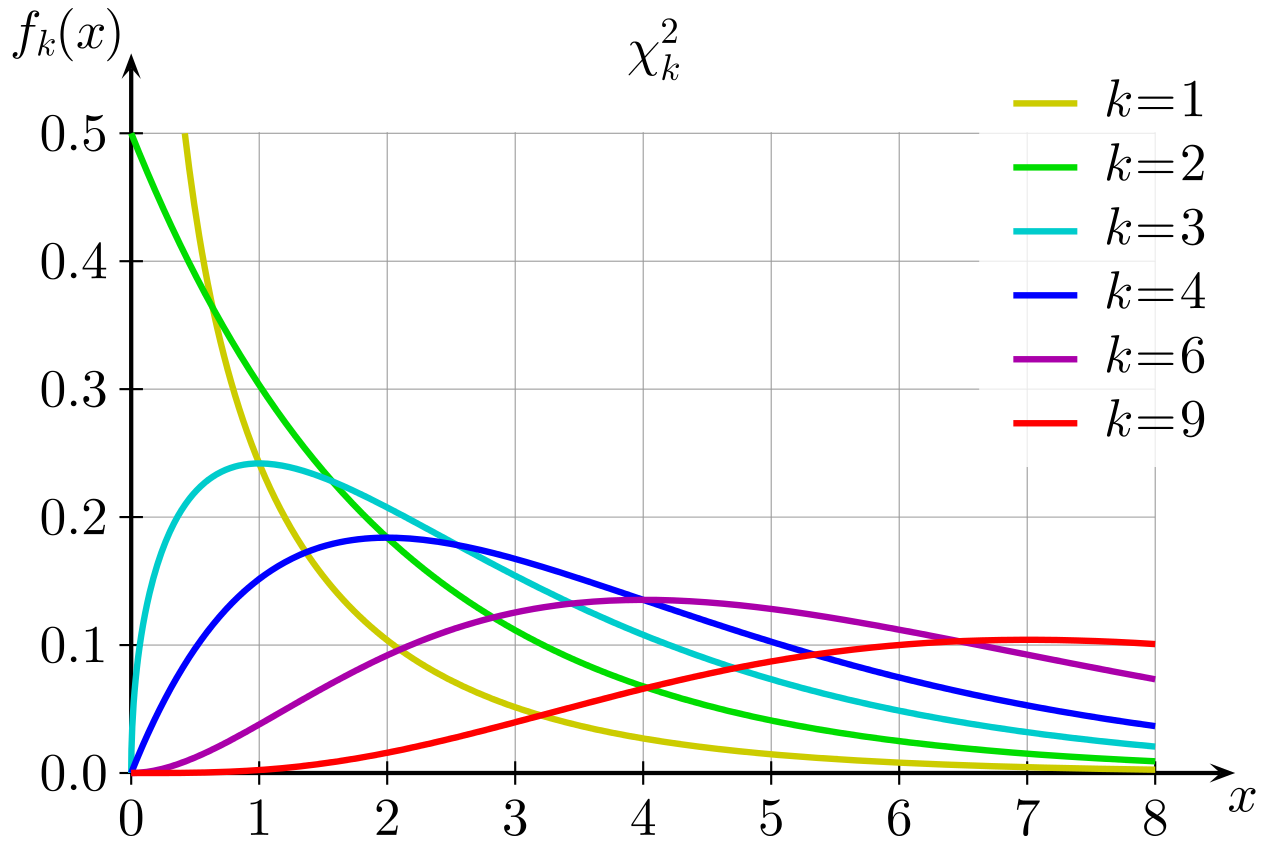
\includegraphics[width=\textwidth]{./Images/chisquared.png}
  \end{minipage}
  \hfill
\begin{minipage}[c]{0.45\textwidth}
 \begin{itemize}
  \item $ \E [X] = k $\\
  $ \E[(X - k)] = 0 $
  \item $ \E [X^2] = k(k+2) $\\
  $ \E[(X - k)^2] = 2k $
  \item $ \E[ X^3] = k(k+2)(k+4) $\\
  $ \E[(X - k)^3] = 8k$ 
  \item $ \E [X^4] = k(k+2)(k+4)(k+6) $\\
  $\E[(X - k)^4] = 12k^2+48k$
 \end{itemize}
\end{minipage}\\

\textbf{Properties}

\begin{itemize}
  \item If $ X_1, \dotsc, X_n $ are independent with $ X_i \sim \chi^2_{p_i} $, then $ \sum X_i \sim \chi^2_{\sum p_i} $ (i.e., independent chi squared variables add to a chi squared, and the degrees of freedom add).
  \item If $ \mX \sim N_n (\mmu, \mSigma) $, then $ (\mX - \mmu)' \mSigma^{-1} (\mX - \mmu) \sim \chi^2_n $.
  \item If $ \mX \sim N_n (\mzero, \mI) $ and $ \mathbf{P}_{n \times n} $ is an idempotent matrix, then $ \mX' \mathbf{P} \mX \sim \chi^2_{rk (\mathbf{P})} = \chi^2_{\operatorname{tr} (\mathbf{P})} $.
  \item If $ \mX \sim N_n (\mzero, \mI) $ then the sum of the squared deviations from the sample mean $ \mX' \mathbf{M}_{\mi} \mX \sim \chi^2_{n-1} $.
\end{itemize}

\subsection*{Student's \( t \)}
PDF: \[ \displaystyle t_\nu = \frac{Z}{\sqrt{X/\nu}} = c\left(1+\frac{x^2}{\nu}\right)^{-\frac{\nu+1}{2}}\] where $Z\sim N(0,1)$, $X\sim \chi^2_\nu$

\begin{minipage}[c]{0.5\textwidth}
  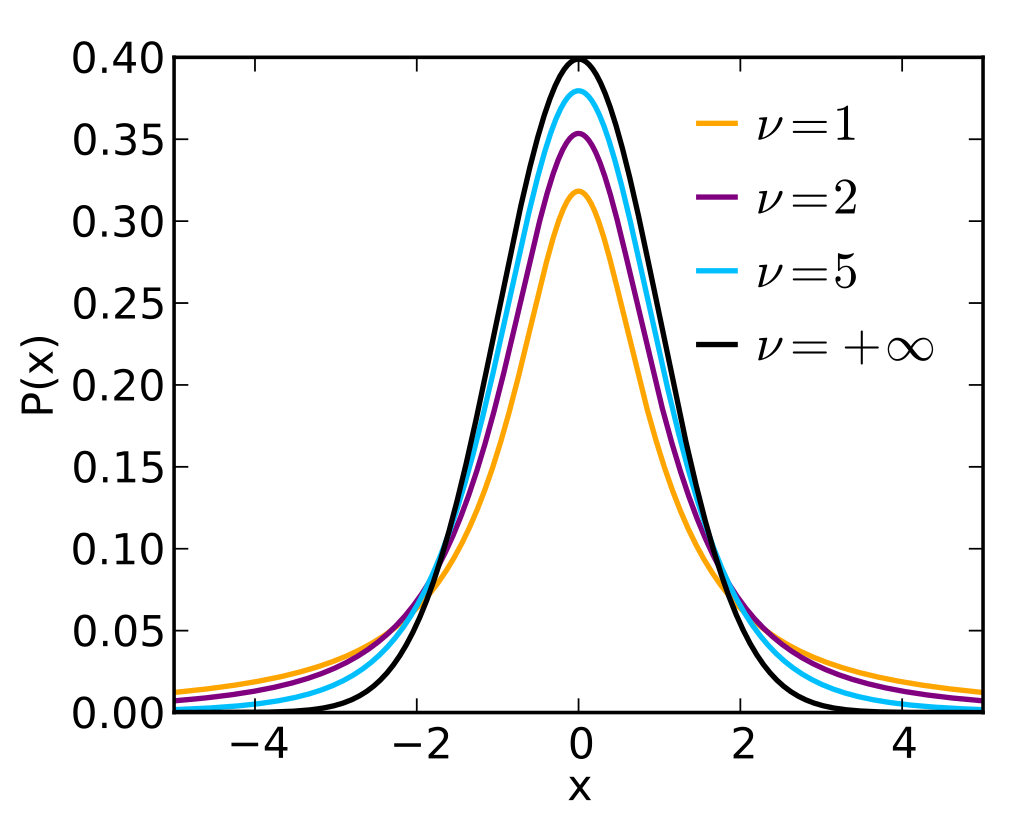
\includegraphics[width=\textwidth]{./Images/tdistribuion.png}
  \end{minipage}
  \hfill
\begin{minipage}[c]{0.45\textwidth}
  \begin{itemize}
    \item Mean: $0$ for $\nu > 1$
    \item Variance: $\frac{\nu}{\nu - 2}$ for $\nu > 2$, $\infty$ for $1 < \nu \leq 2$
    \item Skewness: $0$ for $\nu > 3$
    \item Ex. kurtosis: $\frac{6}{\nu - 4}$ for $\nu > 4$, $\infty$ for $2 < \nu \leq 4$
  \end{itemize}
  
\end{minipage}

\textbf{Why does the $\nu$-th moment of $t_{\nu}$ not exist?}\\
Consider the $\nu$-th raw moment: $\int x^{\nu}c\left(1+\frac{x^2}{\nu}\right)^{-\frac{\nu+1}{2}}dx \approx \int c \nu^{\frac{\nu+1}{2}}x^{-1}dx$ when $x$ is large. This integral diverges, meaning the $\nu$-th raw moment does not exist. A more rigourous proof requires the use of the Beta and Gamma functions.

\textbf{Properties}

\begin{itemize}
  \item If $ X_1, \dotsc, X_n $ are iid $ N (\mu, \sigma^2) $, then $ \sqrt{n} (\bar{X}-\mu) / \sigma \sim N (0,1) $. However, we will generally not know $ \sigma $. Using the sample variance rather than the true variance gives $ \sqrt{n} (\bar{X}-\mu) / s \sim t_{n-1} $.

  \item If a $ t $ distribution has $ \nu $ degrees of freedom, there are only $ \nu-1 $ defined moments. $ \nu $ has thicker tails than normal.
  
  \item$ t_1 $ is Cauchy distribution (the ratio of two independent standard normals). $ t_\infty $ is standard normal.
\end{itemize}

\begin{example}[Derive variance of Student's t]

  Consider $X\sim t_{\nu}$. When \( \nu > 1 \): \[ E(X) = 0 \]
  
  \[ (t_{\nu})^2 \sim F_{1,{\nu}}  \implies E(X^2) = E(Y) \]
  
  with \( Y \sim F_{1,{\nu}} \), where \( F_{1,{\nu}} \) is the F-distribution with \( (1, \nu) \) degrees of freedom. \( E(Y) \) exists if and only if \( \nu > 2 \):
  
  \[ E(Y) = E(X^2) = \frac{\nu}{\nu - 2} \]
  
  We therefore have:
  
  \[ \text{var}(X) = E(X^2) - (E(X))^2 = \frac{\nu}{\nu - 2} \]
  
\end{example}

\subsection*{Snedecor's \( F \)}
PDF: \[ \displaystyle F_{d_1,d_2} = \frac{X_1/d_1}{X_2/d_2}\] where \( X_1 \sim \chi^2_{d_1}\), \( X_2 \sim \chi^2_{d_2}\)

\begin{minipage}[c]{0.5\textwidth}
  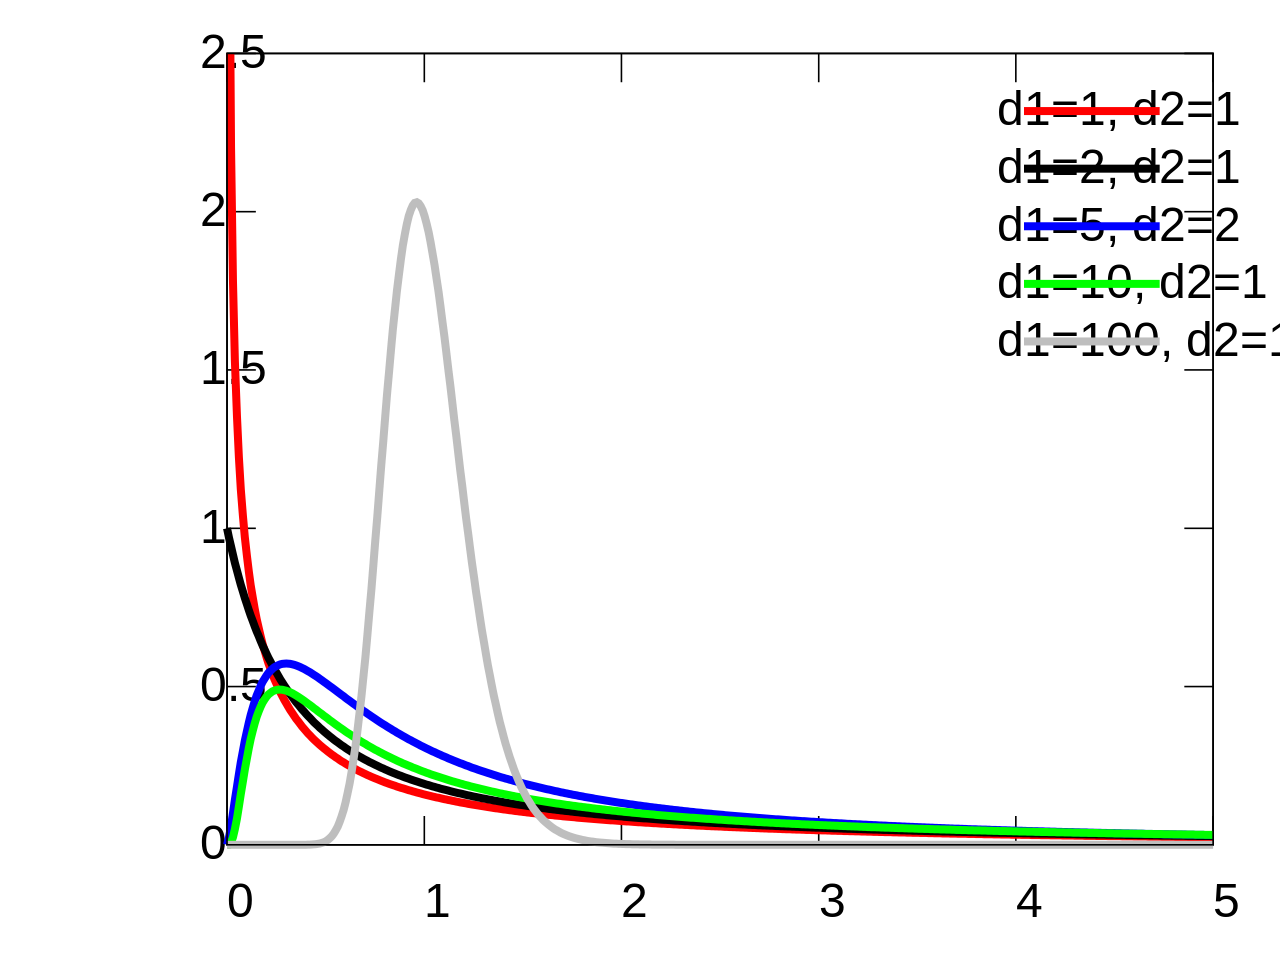
\includegraphics[width=\textwidth]{./Images/fdistribution.png}
  \end{minipage}
  \hfill
\begin{minipage}[c]{0.45\textwidth}
  \begin{itemize}
    \item Mean: $\frac{d_2}{d_2-1}$ for $d_2 > 2$
    \item Variance: $\frac{2 d_2^2 (d_1 + d_2 - 2)}{d_1 (d_2 - 2)^2 (d_2 - 4)}$, for $d_2>4$
  \end{itemize}
\end{minipage}

\textbf{Properties}
\begin{itemize}
  \item $ 1 / F_{p,q} \sim F_{q, p}  $ (i.e., the reciprocal of an $ F $ r.v.\ is another $ F $ with the degrees of freedom switched);
  \item $ (t_q)^2 \sim F_{1,q} $;
  \item If $X \sim F_{p,q}$ then $Y = \lim_{q \to \infty}pX \sim \chi^2_{p}$
\end{itemize}

\section{Conditional expectation function}

\begin{definition}[Conditional distribution]
  Conditional distribution of \( Y \) given \( X \) is defined as

\[ f_{Y|X}(y|x) = \frac{f_{XY}(x, y)}{f_X(x)} \quad \text{if } f_X(x) \neq 0 \]  
\end{definition}
Conditional expectation \( E(Y|X = x) \) is defined as

\[ E(Y|X = x) = \int_{y} y f_{Y|X}(y|x) dy \]

Often, we will skip \( X = x \) having in mind that \( E(Y|X) \) is a function of random variable \( X \). Hence, it is itself a random variable.

We can also condition for/on multiple coordinates: e.g., for $ (X_1, X_2, X_3, X_4) $ a continuous random vector, $ f(x_3, x_4|x_1, x_2) \equiv f(x_1, x_2, x_3, x_4) / f_{X_1 X_2}(x_1, x_2) $, where $ f $ is a joint pdf, and $ f_{X_1 X_2} $ is the marginal pdf in $ X_1 $ and $ X_2 $.

\begin{note}
  \textbf{Borel Paradox}: Be careful when we condition on events of probability zero: two events of probability zero may be equivalent, but the probabilities conditional on the two events is different!
\end{note}

\begin{theorem}[Law of Iterated Expectations]
$ \E X = \E [ \E (X|Y)] $, provided the expectations exist. More generally, when $ \mathcal{L} \subseteq \mathcal{M} $ (i.e., $ \mathcal{L} $ contains less information, $ \mathcal{M} $ contains more),
$$ \E [X | \mathcal{L} ] = \E [ \E (X | \mathcal{M} ) | \mathcal{L} ] = \E [ \E (X | \mathcal{L} ) | \mathcal{M} ] . $$
\end{theorem}

\begin{proof}
  \[
    E(Y) = \int_{y} yf_Y(y)dy = \int_{x} \int_{y} yf_{XY}(x, y)dxdy = \int_{x} \int_{y} yf_{YX}(x, y)dydx
    \]
    \[
    = \int_{x} \int_{y} yf_{Y|X}(y|x)f_X(x)dydx = \int_{x} E(Y|X = x)f_X(x)dx = E(E(Y|X)).
    \]
    
\end{proof}

\begin{theorem}
  $ \E (Y|X) $ is the MSE = $E(Y - g(X))^2$ minimising predictor of $ Y $ based on knowledge of $ X $.
\end{theorem}

\begin{proof}
  \begin{align*}
    E(Y - g(X))^2 &= E[Y - E(Y|X) + E(Y|X) - g(X)]^2 \\
    &= E[Y - E(Y|X)]^2 + 2E[(Y - E(Y|X))(E(Y|X) - g(X))] + E[E(Y|X) - g(X)]^2 
  \end{align*}\\
  Using the law of iterated expectaions: $E(Z) = E(E(Z|X))$
  \begin{align*}
    E[(Y - E(Y|X))(E(Y|X) - g(X))] &= E(E[(Y - E(Y|X))(E(Y|X) - g(X))]|X) \\
    \intertext{Bring terms explained fully by X outside expectation}
    &= E([E(Y|X) - g(X)]E\{[Y - E(Y|X)]|X\}) \\
    \intertext{Expand conditional expectation}
    &= E([E(Y|X) - g(X)]\{E(Y|X) - E(Y|X)\}) \\
    &= 0 \\
    \intertext{Therefore,}
    2E[(Y - E(Y|X))(E(Y|X) - g(X))] &= 0 \implies\\
    E(Y - g(X))^2 &= E[Y - E(Y|X)]^2 + E[E(Y|X) - g(X)]^2 \\
    &\geq E[Y - E(Y|X)]^2.
  \end{align*}\\
    and CEF is the best conditional predictor of \( Y \)
\end{proof}

\begin{lemma}[Leibniz Rule]
  Let \( f(x, t) \) be a continuously differentiable function then, for the function
  \[  F(t) = \int_{a(t)}^{b(t)} f(x, t) \, dx  \]
  the derivative of \( F(t) \) with respect to \( t \) is given by
  \[  \frac{dF}{dt} = \int_{a(t)}^{b(t)} \frac{\partial f}{\partial t} \, dx + f(b(t), t) \cdot \frac{db}{dt} - f(a(t), t) \cdot \frac{da}{dt}  \]
\end{lemma}

\begin{theorem}
  The conditional median $med(Y|X)$ is the expected absolute error = $E(|Y - g(X)||X = x)$ minimizing predictor of $ Y $ based on knowledge of $ X $.
\end{theorem}
The following proof is a complete version of the outline Alexey presents in the notes. A brief (similar) proof is given at the end.\\
\begin{proof}
\begin{align*}
  E(|Y - g(X)||X = x) &= \int_{-\infty}^{\infty} |y - g(x)| f_{Y|X}(y|x) dy\\
  &= \int_{g(x)}^{\infty} (y - g(x)) f_{Y|X}(y|x) dy + \int_{-\infty}^{g(x)} (g(x) - y) f_{Y|X}(y|x) dy.
\end{align*}
Assume that \( f_{Y|X} \) is zero to the left of some constant \( A \), and is unity to the right of some constant \( B \). The problem is: 
\[ \min_{g(x)} \left\{ \phi = \int_{g(x)}^{A} (y - g(x)) f_{Y|X}(y|x) dy + \int_{-B}^{g(x)} (g(x) - y) f_{Y|X}(y|x) dy \right\} \]

Applying Leibniz rule, we have:
\[
\frac{d\phi}{dg(x)} = \int_{A}^{g(x)} (1) f_{Y|X}(y|x) dy + (g(x) - g(x))(1) - (g(x)-A)(0)\]
\[+ \int_{g(x)}^{B} (-1)f_{Y|X}(y|x) dy + (B-g(x))(0) - (g(x)-g(x))(1)
\]

FOC: 
\[
0 =  \int_{A}^{g(x)}f_{Y|X}(y|x) dy -\int_{g(x)}^{B}f_{Y|X}(y|x) dy \implies \int_{A}^{g(x)}f_{Y|X}(y|x) dy = \int_{g(x)}^{B}f_{Y|X}(y|x) dy
\]

Hence, \( g(x) \) must be the value of \( Y \) such that \( P(Y \leq g(x)|X = x) = P(Y > g(x)|X = x) \). That is, \( g(x) \) must be the median of the conditional distribution \( F_{Y|X} \).

To verify that we have minimized \( E(|Y - g(x)||X = x) \):
\[
\frac{d^2\phi}{dg(x)^2} = \frac{\partial}{\partial g(x)} \left( \int_{A}^{g(x)}f_{Y|X}(y|x) dy -\int_{g(x)}^{B}f_{Y|X}(y|x) dy \right)
\]
\[
= \int_{A}^{g(x)} 0f_{Y|X}(y|x) dy + 1\left(\frac{dg(x)}{dg(x)}\right) - 1\left(\frac{dA}{dg(x)}\right)  - \int_{g(x)}^{B} 0f_{Y|X}(y|x) dy + 1\left(\frac{dB}{dg(x)}\right) - 1\left(\frac{dg(x)}{dg(x)}\right)
\]
$=[0+1-0]-[0+0-1]=2(>0)$ so we are characterising a minimum.
\end{proof}
Also, note that if we let \( A \to -\infty \) and \( B \to \infty \), the support of \( F \) can be taken to be the whole real line, so there is no loss of generality in establishing the above result with a support of \( [A, B] \).\\

\textbf{Alternative Proof}
\[\frac{d}{dc} E(|X-c|) = E\left(\frac{d}{dc} |X-c|\right) = E\left(\frac{-(X-c)}{|X-c|}\right)\]
\[= E\left[1_{\{X < c\}} - 1_{\{X > c\}}\right] = P(X < c) - P(X \geq c)\]
\[\frac{d}{dc} E(|X-c|) = 0 \implies P(X < c) = P(X > c) = \frac{1}{2} \]
By definition of the median, $c = med(X)$ \qed\\

\textbf{MAE vs MSE}\\\\
\begin{minipage}[c]{0.5\textwidth}
  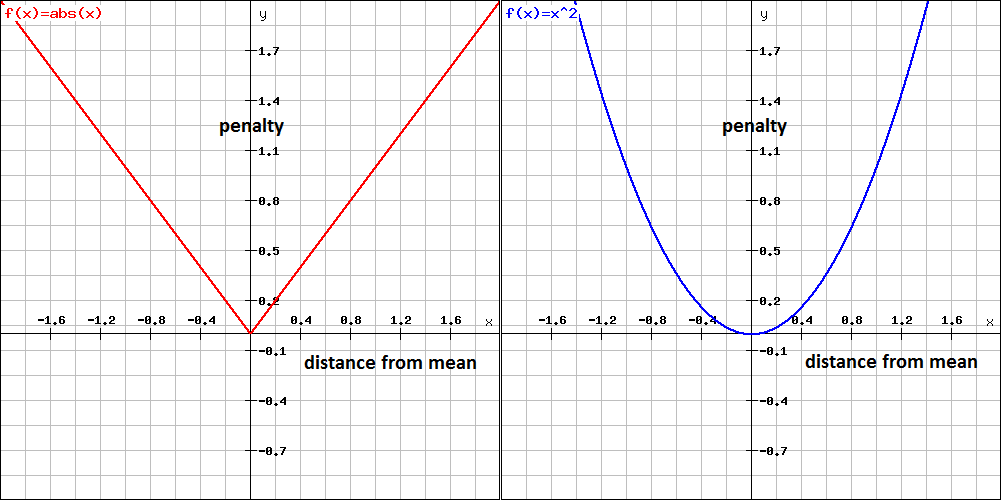
\includegraphics[width=\textwidth]{./Images/msemae.png}
\end{minipage}
  \hfill
\begin{minipage}[c]{0.45\textwidth}
  \begin{itemize}
    \item MAE = $E|Y - g(X)|$
    \item MSE = $E(Y - g(X))^2$
  \end{itemize}
\end{minipage}
\begin{itemize}
  \item MAE imposes a linear penalty on errors, i.e.: each deviation from the mean is given a proportional corresponding error. 
  \item MSE is a squared proportional relationship between deviation and penalty. This will make sure that the further you are away from the mean, the proportionally more you will be penalized. Using this penalty function, outliers are deemed proportionally more informative than observations near the mean.
\end{itemize}
Because the MAE is a more robust estimator of scale than the sample variance or standard deviation, it works better with distributions without a mean or variance, such as the Cauchy distribution. \\

\textbf{Weighted MAE}\\
If underprediction is marginally less or more costly as overprediction, it makes sense to minimize the expectation of
\[
\tau 1(Y > g(X))(Y - g(X)) + (1 - \tau) 1(Y \leq g(X))(g(X) - Y)
\]
with \( \tau \in (0, 1) \). For example, parameter \( \tau < 1/2 \) would correspond to situations where the underprediction is less costly than overprediction. Following the same logic as above, we can show that \textit{the corresponding best predictor would be \( \tau \)-th quantile \( \tau(X) \) of the conditional distribution of \( Y \) given \( X \)}.\\
Below we have (from left to right): $\tau$ = 1 (no cost to overprediction), $\tau$ = 0 (no cost to underprediction) and $\tau$ = 0.3 (cost to both, but relatively more to overprediction.)\\\\
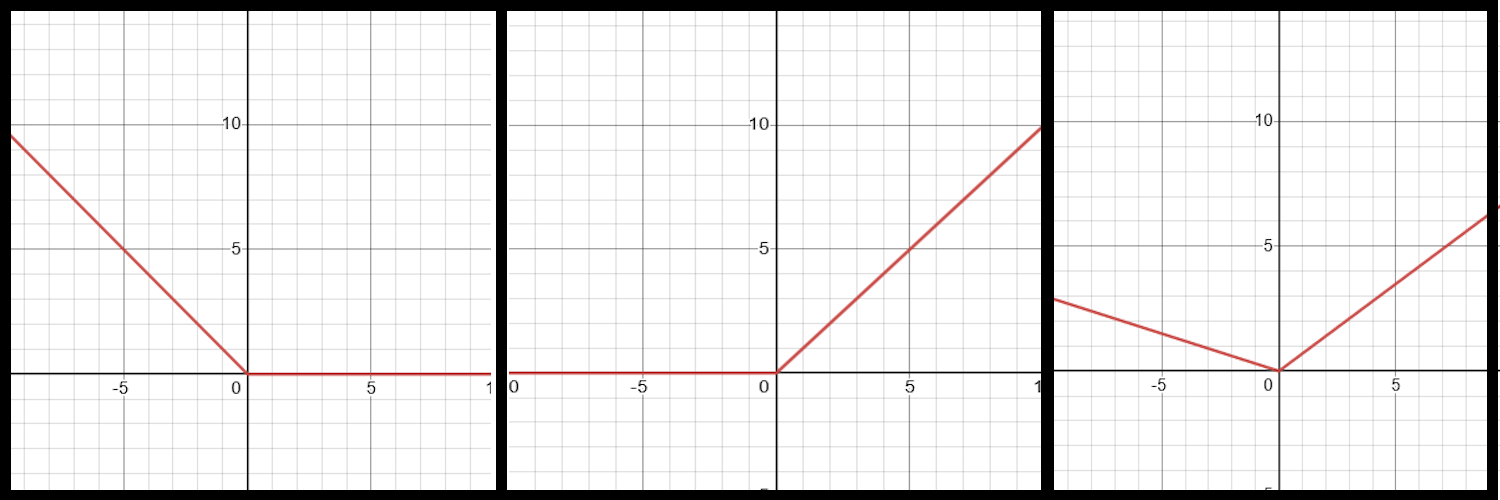
\includegraphics[width=\textwidth]{./Images/weightedMAD.png}


\end{document}
